\documentclass[tikz,border=8pt]{standalone}
\usepackage{amsmath}
\usepackage{amssymb}
\usepackage{xcolor}
\usetikzlibrary{arrows.meta,positioning}

\definecolor{predictoraccent}{HTML}{1F77B4} % Matplotlib C0
\definecolor{sharedaccent}{HTML}{2CA02C}    % Matplotlib C2
\definecolor{responseaccent}{HTML}{FF7F0E} % Matplotlib C1
\definecolor{observedfill}{HTML}{F4F5F7}
\definecolor{noisefill}{HTML}{E9EBEF}
\definecolor{textgray}{HTML}{30343B}

\tikzset{
  latent/.style={
    rounded corners=3pt,
    minimum width=3.6cm,
    minimum height=1.45cm,
    align=center,
    line width=0.8pt,
    text=textgray,
  },
  observed/.style={
    rounded corners=3pt,
    minimum width=3.6cm,
    minimum height=1.35cm,
    align=center,
    draw=textgray,
    fill=observedfill,
    line width=0.9pt,
    text=textgray,
  },
  noise/.style={
    rounded corners=2pt,
    inner xsep=8pt,
    inner ysep=5pt,
    draw=textgray!70,
    fill=noisefill,
    line width=0.7pt,
    text=textgray,
  },
  signal/.style={
    -{Latex[length=2.4mm,width=1.6mm]},
    line width=1.0pt,
  },
  noise arrow/.style={
    -{Latex[length=2.2mm,width=1.5mm]},
    line width=0.8pt,
    draw=textgray!75,
  },
  edge label/.style={
    fill=white,
    inner sep=1.5pt,
    text=textgray,
    font=\small,
  },
}

\begin{document}
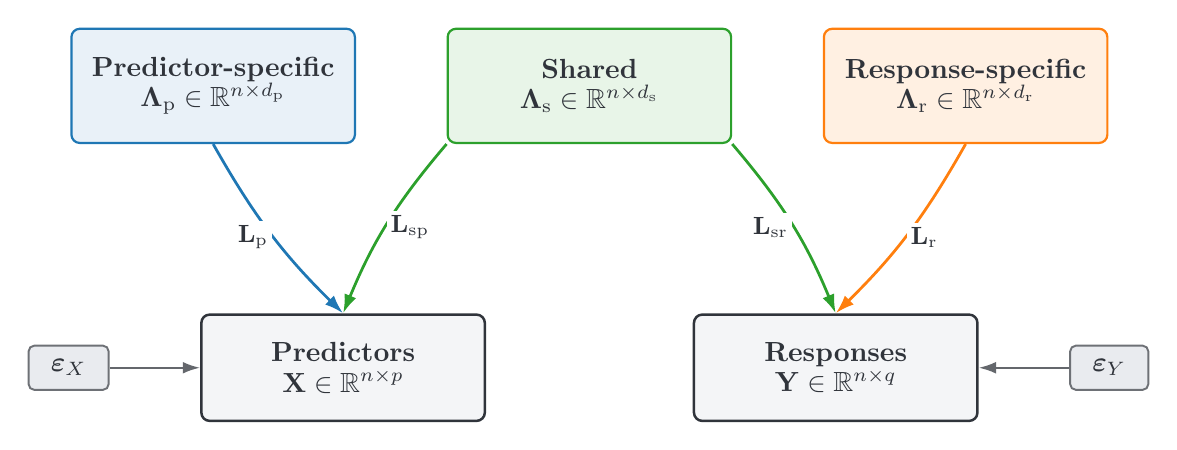
\begin{tikzpicture}[node distance=1.35cm and 1.15cm]
  \node[latent, draw=predictoraccent, fill=predictoraccent!10] (pred) {
    \textbf{Predictor-specific}\\[-1pt]
    $\boldsymbol{\Lambda}_{\mathrm{p}}\in\mathbb{R}^{n\times d_{\mathrm{p}}}$
  };
  \node[latent, draw=sharedaccent, fill=sharedaccent!11, right=of pred] (shared) {
    \textbf{Shared}\\[-1pt]
    $\boldsymbol{\Lambda}_{\mathrm{s}}\in\mathbb{R}^{n\times d_{\mathrm{s}}}$
  };
  \node[latent, draw=responseaccent, fill=responseaccent!12, right=of shared] (resp) {
    \textbf{Response-specific}\\[-1pt]
    $\boldsymbol{\Lambda}_{\mathrm{r}}\in\mathbb{R}^{n\times d_{\mathrm{r}}}$
  };

  \node[observed, below=2.15cm of pred, xshift=1.65cm] (x) {
    \textbf{Predictors}\\[-1pt]
    $\mathbf{X}\in\mathbb{R}^{n\times p}$
  };
  \node[observed, below=2.15cm of resp, xshift=-1.65cm] (y) {
    \textbf{Responses}\\[-1pt]
    $\mathbf{Y}\in\mathbb{R}^{n\times q}$
  };

  \node[noise, left=1.15cm of x] (epsx) {$\boldsymbol{\varepsilon}_{X}$};
  \node[noise, right=1.15cm of y] (epsy) {$\boldsymbol{\varepsilon}_{Y}$};

  \draw[signal, draw=predictoraccent]
    (pred.south) to[bend right=8]
    node[edge label, pos=0.52, left] {$\mathbf{L}_{\mathrm{p}}$} (x.north);

  \draw[signal, draw=sharedaccent]
    (shared.south west) to[bend right=9]
    node[edge label, pos=0.52, right] {$\mathbf{L}_{\mathrm{sp}}$} (x.north);

  \draw[signal, draw=sharedaccent]
    (shared.south east) to[bend left=9]
    node[edge label, pos=0.52, left] {$\mathbf{L}_{\mathrm{sr}}$} (y.north);

  \draw[signal, draw=responseaccent]
    (resp.south) to[bend left=8]
    node[edge label, pos=0.52, right] {$\mathbf{L}_{\mathrm{r}}$} (y.north);

  \draw[noise arrow] (epsx.east) -- (x.west);
  \draw[noise arrow] (epsy.west) -- (y.east);
\end{tikzpicture}
\end{document}
